% prediccion_rls.tex — revisión del predictor de trayectoria (IEE2913, Grupo 9), 17-11-2026
% Compilar con XeLaTeX (dos pasadas):  xelatex prediccion_rls.tex
% Las figuras se generan con docs/figuras/figuras_prediccion.py
\documentclass[11pt,a4paper]{article}
\usepackage[a4paper,margin=2.3cm,top=2.2cm,bottom=2.4cm]{geometry}
\usepackage{fontspec}
\usepackage{polyglossia}
\setdefaultlanguage{spanish}
\gappto\captionsspanish{\renewcommand{\tablename}{Tabla}}
\setmonofont{DejaVu Sans Mono}[Scale=0.80]
\usepackage{amsmath,amssymb}
\usepackage{graphicx}
\usepackage{booktabs,array,tabularx}
\usepackage{xcolor}
\usepackage{enumitem}
\usepackage{fancyvrb}
\usepackage{caption}
\usepackage{float}
\usepackage{titlesec}
\usepackage{fancyhdr}
\usepackage{tikz}
\usetikzlibrary{positioning,arrows.meta}
\usepackage[most]{tcolorbox}
\usepackage[hidelinks]{hyperref}

\graphicspath{{figuras/}}

\definecolor{tinta}{HTML}{0B0B0B}
\definecolor{tintados}{HTML}{52514E}
\definecolor{tenue}{HTML}{898781}
\definecolor{azul}{HTML}{2A78D6}
\definecolor{azulosc}{HTML}{184F95}
\definecolor{naranja}{HTML}{EB6834}
\definecolor{fondo}{HTML}{F4F7FC}
\definecolor{fondogris}{HTML}{F6F5F2}
\definecolor{regla}{HTML}{C3C2B7}

\color{tinta}
\setlength{\parindent}{0pt}
\setlength{\parskip}{0.55em}
\emergencystretch=2em
\setlist{itemsep=0.2em,topsep=0.25em,parsep=0.1em,leftmargin=1.5em}
\captionsetup{font=small,labelfont=bf,labelsep=period,skip=5pt}
\titleformat{\section}{\Large\bfseries\color{azulosc}}{\thesection.}{0.5em}{}
\titleformat{\subsection}{\large\bfseries}{\thesubsection}{0.5em}{}
\titlespacing*{\section}{0pt}{1.4em}{0.5em}
\titlespacing*{\subsection}{0pt}{1.0em}{0.3em}
\pagestyle{fancy}
\fancyhf{}
\renewcommand{\headrulewidth}{0pt}
\fancyfoot[L]{\small\color{tenue}IEE2913 · Grupo 9 · Predictor de trayectoria RLS}
\fancyfoot[R]{\small\color{tenue}\thepage}

\newcommand{\cod}[1]{\texttt{#1}}
\newcommand{\lam}{\lambda}
\newcommand{\gr}{^{\circ}}
\newtcolorbox{clave}[1][]{enhanced,breakable,colback=fondo,colframe=azul,boxrule=0pt,leftrule=3pt,
  arc=0pt,left=9pt,right=9pt,top=6pt,bottom=6pt,before skip=0.8em,after skip=0.8em,fonttitle=\bfseries,
  coltitle=azulosc,colbacktitle=fondo,titlerule=0pt,attach title to upper={\par\smallskip},#1}
\newtcolorbox{lamina}[1]{enhanced,colback=white,colframe=regla,boxrule=0.6pt,arc=3pt,left=10pt,right=10pt,
  top=5pt,bottom=5pt,before skip=0.45em,after skip=0.45em,fonttitle=\bfseries,coltitle=azulosc,
  colbacktitle=white,titlerule=0pt,attach title to upper={\par\smallskip},title={#1}}
\DefineVerbatimEnvironment{codigo}{Verbatim}{fontsize=\small,frame=leftline,framerule=1.2pt,
  rulecolor=\color{regla},framesep=8pt,xleftmargin=4pt,baselinestretch=1.02}

\begin{document}

% ------------------------------------------------------------------------------------------
{\color{azulosc}\rule{\linewidth}{1.4pt}}

\vspace{0.5em}
{\LARGE\bfseries Predictor de trayectoria RLS}\\[0.35em]
{\large Teoría, implementación y ajuste — \cod{pt/rls\_predictor.py} y \cod{pt/prediccion.py}}\\[0.5em]
{\small\color{tintados}IEE2913 Diseño Eléctrico (Capstone) · Grupo 9 · Plataforma pan-tilt \hfill Revisión del 17-11-2026}

\vspace{0.2em}
{\color{regla}\rule{\linewidth}{0.5pt}}

\begin{clave}[title={Lo esencial}]
\begin{itemize}[leftmargin=1.2em]
  \item \textbf{Qué hace.} En cada cuadro ajusta una parábola a las últimas posiciones del objetivo y la evalúa
        unos 20~ms más adelante: el instante en que el ESP32 recibirá la consigna. Así la plataforma apunta a
        donde el objetivo \emph{va a estar}, no a donde estaba en la foto.
  \item \textbf{El núcleo está bien.} Con orden 3 y $\lam = 0{,}80$ el error de predicción simulado es unas diez veces
        menor que sin predictor ($0{,}045\gr$ contra $0{,}45\gr$, objetivo a $31\gr$/s como máximo).
  \item \textbf{Por qué ``funciona más o menos''.} En el lazo cerrado simulado, \emph{sin} feedforward de velocidad
        el error de centrado casi no depende de $\lam$: unos 28~px en régimen para cualquier valor. Lo domina el
        atraso del lazo de posición del ESP32, no el predictor. Con feedforward baja a 2,3~px.
  \item \textbf{Efecto de $\lam$.} Subirlo filtra más el ruido y hace al predictor más lento ante maniobras;
        bajarlo lo hace rápido y ruidoso. Rango útil con orden 3: de 0,75 a 0,88.
  \item \textbf{Qué cambiar primero.} (1)~Activar el feedforward. (2)~Medir el ruido real de la medición y elegir
        $\lam$ con la tabla~\ref{tab:mejor}. (3)~Corregir la cadena reinicio $\rightarrow$ confianza 0
        $\rightarrow$ PÉRDIDA. El detalle está en la sección~\ref{sec:ajustes}.
\end{itemize}
\end{clave}

{\small\color{tintados}Las cifras de este documento vienen de simulaciones con el código real del predictor y con
el modelo de planta de \cod{pid\_t\_2} (amortiguamiento supuesto $\zeta = 0{,}05$). No son mediciones de la
plataforma. Se reproducen con \cod{docs/figuras/figuras\_prediccion.py} y
\cod{herramientas/barrido\_lazo\_cerrado.py}.}

% ------------------------------------------------------------------------------------------
\section{Para qué sirve y dónde está}

Entre la exposición de un cuadro y la llegada de la consigna al ESP32 pasan unos 12 a 19~ms: lectura del
sensor, detección, cálculo y enlace serie. En ese tiempo un objetivo a $30\gr$/s avanza $0{,}5\gr$, más de
4~px de la imagen. El predictor compensa ese retardo y, además, entrega la \emph{velocidad} del objetivo,
que se puede enviar al ESP32 como feedforward.

\begin{table}[H]
\centering\small
\begin{tabularx}{\linewidth}{@{}l>{\raggedright\arraybackslash}X@{}}
\toprule
Archivo & Qué contiene \\
\midrule
\cod{pt/rls\_predictor.py} & \cod{PredictorRLS}: el estimador de un eje. Mínimos cuadrados recursivos con factor de olvido sobre un polinomio local. \\
\cod{pt/prediccion.py} & \cod{EstimadorEje}: envuelve al RLS con el rechazo de mediciones aberrantes (\emph{gating}) y el reinicio. \cod{Estimador2D}: dos ejes, horizonte de predicción y confianza. \\
\cod{pt/control.py} & \cod{ReferenciaVisual}: convierte la detección en dirección del mundo, llama al estimador y arma la consigna ($\theta_{\mathrm{ref}}$ y $\omega_{\mathrm{ff}}$). \\
\cod{pt/parametros.py} & \cod{Prediccion}: orden, $\lam$, gating, tiempos de oclusión y confianza. \\
\bottomrule
\end{tabularx}
\end{table}

\begin{figure}[H]
\centering
\begin{tikzpicture}[font=\footnotesize, node distance=4.5mm,
  caja/.style={draw=regla, rounded corners=2pt, fill=fondogris, align=center, inner sep=4pt, minimum height=11mm, text width=20mm},
  pred/.style={caja, draw=azul, fill=fondo, line width=0.9pt},
  fl/.style={-{Stealth[length=4.5pt]}, draw=tintados, line width=0.5pt}]
  \node[caja] (cam) {Cámara\\80 cuadros/s};
  \node[caja, right=of cam] (det) {Detección\\$(u, w)$ en píxeles};
  \node[caja, right=of det] (geo) {Geometría\\dirección en el mundo [$\gr$]};
  \node[pred, right=of geo] (rls) {\textbf{Predictor}\\gating + RLS por eje};
  \node[caja, right=15mm of rls] (esp) {ESP32\\lazo PI a 1~kHz};
  \draw[fl] (cam) -- (det);
  \draw[fl] (det) -- (geo);
  \draw[fl] (geo) -- (rls);
  \draw[fl] (rls) -- node[above, font=\scriptsize] {$\theta_{\mathrm{ref}},\ \omega_{\mathrm{ff}}$} (esp);
  \draw[fl] (esp.south) -- ++(0,-6mm) -| node[pos=0.25, below, font=\scriptsize] {$\theta_{\mathrm{med}}$ del AS5600 en el instante de la foto} (geo.south);
\end{tikzpicture}
\caption{Lugar del predictor en el lazo externo. Trabaja en ángulos del mundo (pan y tilt del objetivo), no en
píxeles: en la imagen, el movimiento del objetivo se mezcla con el de la propia plataforma.}
\end{figure}

\begin{figure}[H]
\centering
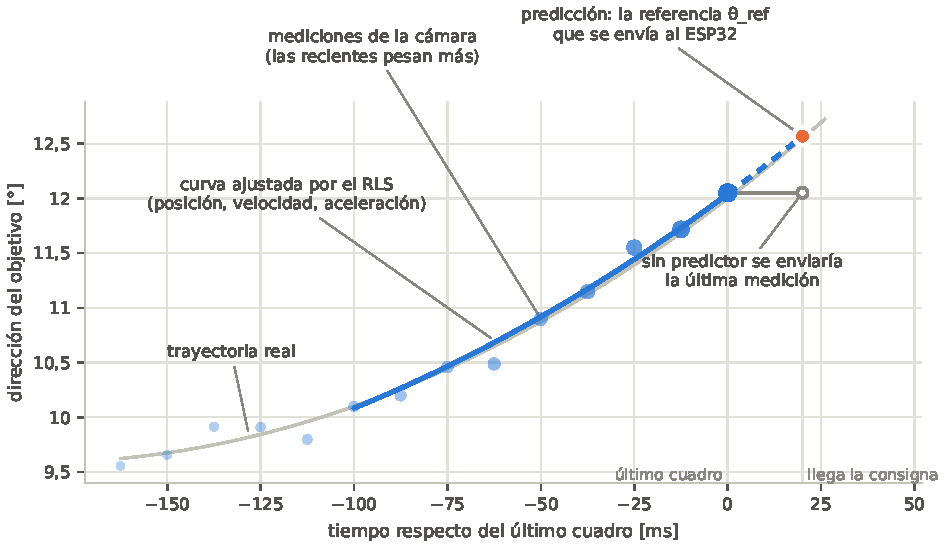
\includegraphics[width=0.94\linewidth]{pred_concepto.pdf}
\caption{La idea, con el código real (orden 3, $\lam = 0{,}80$, ruido exagerado a $0{,}10\gr$ para que se vea).
El tamaño de cada punto es su peso en el ajuste. La línea segmentada es la extrapolación de 20~ms.}
\label{fig:concepto}
\end{figure}

% ------------------------------------------------------------------------------------------
\section{Teoría}

\subsection{Modelo: un polinomio local por eje}

Cada eje (pan y tilt) se trata por separado. Cerca del instante actual $t_0$, la dirección del objetivo se
aproxima con un polinomio en $s = t - t_0$:
\begin{equation}
  y(t_0 + s) \;=\; \theta_0 + \theta_1\, s + \theta_2\, s^2 \;=\; \boldsymbol{\varphi}(s)^{\mathsf T}\boldsymbol{\theta},
  \qquad \boldsymbol{\varphi}(s) = \begin{bmatrix} 1 & s & s^2 \end{bmatrix}^{\mathsf T}.
  \label{eq:modelo}
\end{equation}
Con el origen puesto en la última muestra, los parámetros tienen significado físico directo: $\theta_0$ es la
posición, $\theta_1$ la velocidad y $2\theta_2$ la aceleración. El \emph{orden} $n$ del código es el número de
parámetros: $n = 2$ supone velocidad constante y $n = 3$ agrega la aceleración.

\subsection{Mínimos cuadrados con factor de olvido}

Los parámetros se eligen para minimizar el error cuadrático de las mediciones $y_k$, dando menos peso a las
más antiguas. Si $N$ es el cuadro actual:
\begin{equation}
  J(\boldsymbol{\theta}) \;=\; \sum_{k=1}^{N} \lam^{\,N-k}\,\bigl(y_k - \boldsymbol{\varphi}_k^{\mathsf T}\boldsymbol{\theta}\bigr)^2,
  \qquad 0 < \lam < 1 .
  \label{eq:costo}
\end{equation}
El cuadro actual pesa 1, el anterior $\lam$, el de antes $\lam^2$, y así sucesivamente. La suma de todos los
pesos es la \textbf{memoria efectiva}:
\begin{equation}
  N_{\mathrm{ef}} = \frac{1}{1-\lam}\ \text{cuadros}, \qquad \tau_{\mathrm{mem}} = \frac{T}{1-\lam},
  \label{eq:memoria}
\end{equation}
con $T = 12{,}5$~ms a 80 cuadros por segundo. Con $\lam = 0{,}80$ son 5~cuadros, es decir 62,5~ms.

\subsection{Forma recursiva}

Resolver \eqref{eq:costo} desde cero en cada cuadro sería caro. El RLS llega al mismo resultado actualizando
la solución anterior con la medición nueva. Guarda dos cosas: el vector $\boldsymbol{\theta}$ y la matriz
$\mathbf P$, que es la covarianza de los parámetros (cuánta incertidumbre queda en cada uno). Por cada
medición $y$ tomada en $s$:
\begin{align}
  \mathbf k &= \frac{\mathbf P\,\boldsymbol{\varphi}}{\lam + \boldsymbol{\varphi}^{\mathsf T}\mathbf P\,\boldsymbol{\varphi}} && \text{ganancia: cuánto creerle a la medición} \label{eq:k}\\
  e &= y - \boldsymbol{\varphi}^{\mathsf T}\boldsymbol{\theta} && \text{innovación: lo que la medición no calza con lo previsto} \label{eq:e}\\
  \boldsymbol{\theta} &\leftarrow \boldsymbol{\theta} + \mathbf k\, e && \text{corrección de los parámetros} \label{eq:th}\\
  \mathbf P &\leftarrow \frac{\mathbf P - \mathbf k\,\boldsymbol{\varphi}^{\mathsf T}\mathbf P}{\lam} && \text{menos incertidumbre por medir; más por olvidar} \label{eq:P}
\end{align}
Dividir por $\lam$ en \eqref{eq:P} es lo que implementa el olvido: infla la incertidumbre en cada paso, de modo
que la ganancia $\mathbf k$ nunca llega a cero y el estimador sigue atento a los cambios.

\subsection{Traslado del origen}

Si $s$ se midiera desde el primer cuadro, crecería sin límite y $s^2$ arruinaría el condicionamiento numérico
de $\mathbf P$. Por eso, después de cada actualización el origen se traslada a la muestra recién incorporada.
Reescribir el mismo polinomio con otro origen es un cambio lineal de parámetros:
\begin{equation}
  \boldsymbol{\theta}' = \mathbf A(s)\,\boldsymbol{\theta}, \qquad \mathbf P' = \mathbf A(s)\,\mathbf P\,\mathbf A(s)^{\mathsf T},
  \qquad
  \mathbf A(s) = \begin{bmatrix} 1 & s & s^2 \\ 0 & 1 & 2s \\ 0 & 0 & 1 \end{bmatrix}.
  \label{eq:A}
\end{equation}
El polinomio no cambia; sólo cambia desde dónde se mide $s$. Así el regresor siempre se evalúa con $s$ del
orden de un período de cuadro, y el método acepta sin problema que los cuadros no lleguen equiespaciados.

\subsection{Predicción, velocidad y oclusiones}

\begin{itemize}
  \item \textbf{Predicción} en un instante futuro $t$: $\hat y(t) = \boldsymbol{\varphi}(t - t_0)^{\mathsf T}\boldsymbol{\theta}$.
  \item \textbf{Velocidad} en ese instante (derivada del polinomio): $\hat v(t) = \theta_1 + 2\,\theta_2\,(t - t_0)$.
  \item \textbf{Sin medición} (oclusión o detección inválida): no hay corrección. Sólo se aplica
        $\mathbf P \leftarrow \mathbf P/\lam$, de modo que la incertidumbre crece y la primera medición que
        vuelva pesa mucho. Mientras tanto la predicción es pura extrapolación del último polinomio.
\end{itemize}

% ------------------------------------------------------------------------------------------
\section{Implementación}

\subsection{\cod{rls\_predictor.py}: el estimador de un eje}

La clase \cod{PredictorRLS} guarda \cod{th} ($\boldsymbol{\theta}$), \cod{P}, \cod{t0} (origen del polinomio) y
\cod{n\_valid} (muestras válidas). El método \cod{actualizar(t, y, valido)} es la traducción directa de las
ecuaciones \eqref{eq:k} a \eqref{eq:A}:

\begin{codigo}
s = t - self.t0                      # tiempo desde la última muestra
if not valido:
    self.P = self.P / self.lam       # oclusión: sólo crece la incertidumbre
    self._sanear();  return None
phi  = self._phi(s)                  # [1, s, s²]
Pphi = self.P @ phi
k    = Pphi / (self.lam + phi @ Pphi)            # ganancia          (ec. 4)
e    = y - phi @ self.th                         # innovación        (ec. 5)
self.th = self.th + k * e                        # corrección        (ec. 6)
self.P  = (self.P - np.outer(k, Pphi)) / self.lam    # covarianza    (ec. 7)
self._sanear()
A = self._A(s)                       # traslado del origen a esta muestra (ec. 8)
self.th = A @ self.th;  self.P = A @ self.P @ A.T;  self.t0 = t
\end{codigo}

Tres detalles de la implementación:
\begin{itemize}
  \item \textbf{Arranque.} \cod{P} parte en $\delta\,\mathbf I$ con $\delta = 10^4$ (``no sé nada''), y la primera
        muestra sólo fija $\theta_0$. \cod{listo()} es verdadero cuando hay al menos $n$ muestras válidas; antes
        no hay datos para estimar velocidad ni aceleración.
  \item \textbf{\cod{\_sanear()}.} Fuerza la simetría de $\mathbf P$ (los errores de redondeo la rompen de a poco) y
        limita su traza a $10^6$. Ese tope evita que $\mathbf P$ crezca sin control durante una oclusión larga.
  \item \textbf{\cod{predecir(t)}} evalúa el polinomio en el instante absoluto $t$. La velocidad se calcula
        aparte, en \cod{EstimadorEje.velocidad()}, con los mismos parámetros y sin tocar esta clase.
\end{itemize}

\subsection{\cod{prediccion.py}: gating, reinicio y confianza}

\cod{EstimadorEje} protege al RLS de las mediciones malas. Antes de incorporar una medición calcula la
innovación $e = y - \hat y$ y la compara con un umbral:
\begin{equation}
  |e| \;>\; k_g \cdot \max(\sigma,\ \sigma_{\min}) \quad\Longrightarrow\quad \text{medición rechazada.}
\end{equation}
\begin{itemize}
  \item $\sigma$ es un promedio móvil de $|e|$ (90~\% del valor anterior, 10~\% del nuevo): el tamaño típico
        del error de un cuadro al siguiente.
  \item Valores actuales: $k_g = 6$ y $\sigma_{\min} = 0{,}1\gr$. El umbral nunca baja de $0{,}6\gr$, unos 5~px.
  \item Una medición rechazada no entra al RLS. Tras \cod{max\_rechazos} $= 3$ rechazos seguidos se asume que
        no era un aberrante sino una maniobra real, y el estimador \textbf{se reinicia} con esa medición.
\end{itemize}

\cod{Estimador2D} junta los dos ejes y hace tres cosas más:
\begin{itemize}
  \item \textbf{Tiempo relativo.} Resta el instante del primer cuadro, para no operar con números grandes.
  \item \textbf{Horizonte.} Predice en el instante absoluto que le pasan (\cod{t\_pred\_s}); el valor fijo
        \cod{horizonte\_s} sólo se usa si no se lo pasan.
  \item \textbf{Confianza} entre 0 y 1: vale 0 si el estimador todavía no está listo o si lleva más de
        \cod{t\_max\_s} $= 0{,}5$~s sin medición; si no, $e^{-t_{\mathrm{sin}}/\tau}$ con $\tau = 0{,}2$~s. El
        supervisor pasa a PÉRDIDA cuando baja de 0,2.
\end{itemize}

\subsection{Cómo se usa en el lazo}

\begin{enumerate}
  \item \textbf{Medición.} \cod{ReferenciaVisual.actualizar()} convierte $(u, w)$ en dirección del mundo con
        la pose de la plataforma en el instante de la foto. Ese instante es el de la \emph{fila} donde está el
        objetivo, porque el sensor lee fila por fila (persiana rodante).
  \item \textbf{Horizonte.} \cod{main.py} calcula $t_{\mathrm{aplic}} = t_{\mathrm{envío}} + 1$~ms (retardo del
        enlace) y pide la predicción en ese instante. El horizonte no es una constante: es el retardo real de
        cada cuadro, y queda en la columna \cod{h\_ms} del registro.
  \item \textbf{Consigna.} En SEGUIMIENTO, $\theta_{\mathrm{ref}}$ es la predicción, limitada al recorrido. Si el
        feedforward está activo, $\omega_{\mathrm{ff}}$ es la velocidad estimada en $t_{\mathrm{aplic}}$. Fuera de
        SEGUIMIENTO se retiene la última referencia.
  \item \textbf{ESP32.} Calcula $e = \theta_{\mathrm{ref}} - \theta_{\mathrm{med}}$ y aplica el PI. Con feedforward,
        suma $\omega_{\mathrm{ff}}$ a la salida del PI y hace avanzar la referencia entre consignas.
\end{enumerate}

% ------------------------------------------------------------------------------------------
\section{Efecto de \texorpdfstring{$\lam$}{lambda}}
\label{sec:lambda}

\begin{clave}[title={¿Qué pasa al aumentar o disminuir $\lam$?}]
\begin{tabularx}{\linewidth}{@{}>{\raggedright\arraybackslash}p{3.1cm}>{\raggedright\arraybackslash}X>{\raggedright\arraybackslash}X@{}}
 & \textbf{Aumentar $\lam$} (hacia 0,95) & \textbf{Disminuir $\lam$} (hacia 0,60) \\[2pt]
Memoria & Larga: promedia más cuadros & Corta: usa sólo los últimos \\
Ruido en $\theta_{\mathrm{ref}}$ y $\omega_{\mathrm{ff}}$ & Baja & Sube; con orden 3, bajo 0,75 la predicción es más ruidosa que la medición \\
Ante una maniobra & Reacciona lento y se pasa de largo antes de asentarse & Reacciona de inmediato \\
Objetivo que acelera & Aparece un error sistemático (atraso) & Lo sigue bien \\
Tras un reinicio & Tarda más en converger & Converge en pocos cuadros \\
\end{tabularx}
\end{clave}

$\lam$ no filtra en el tiempo como un pasa-bajos sobre la posición: decide \emph{cuántos cuadros} entran al
ajuste del polinomio. Con muchos cuadros el ajuste promedia el ruido, pero supone que la misma parábola vale
para todo ese tramo. Si el objetivo cambió de movimiento dentro de la ventana, el ajuste queda atrasado.

\begin{figure}[H]
\centering
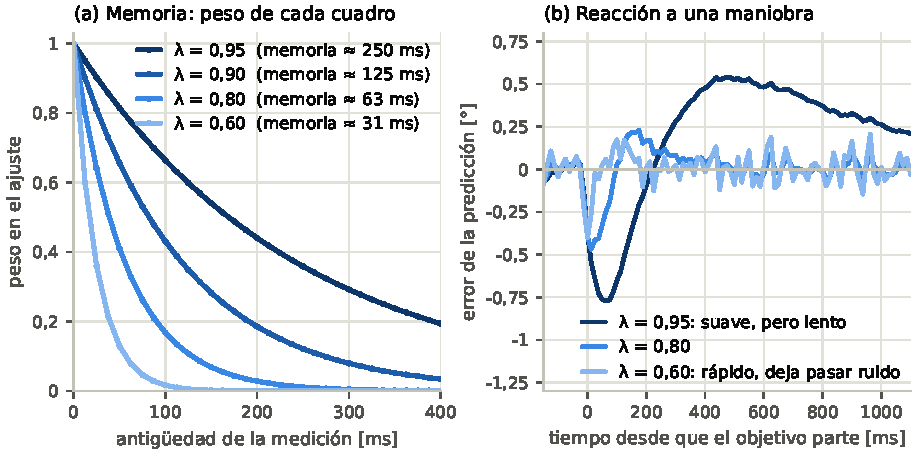
\includegraphics[width=\linewidth]{pred_lambda.pdf}
\caption{(a) Peso de cada cuadro según su antigüedad. (b) Error de la predicción a 20~ms cuando un objetivo
quieto parte a $20\gr$/s en $t = 0$ (orden 3, ruido de $0{,}05\gr$, la misma realización de ruido para los tres).
Con $\lam = 0{,}80$ el error vuelve a cero en unos 250~ms; con $0{,}95$ llega a $0{,}77\gr$ y sigue con error
un segundo después.}
\label{fig:lambda}
\end{figure}

La tabla~\ref{tab:ruido} cuantifica el lado del ruido. La ganancia de posición es la razón entre la desviación
estándar de la predicción y la de la medición $\sigma$; la de velocidad multiplica a $\sigma$ para dar el ruido
de $\omega_{\mathrm{ff}}$.

\begin{table}[H]
\centering\small
\caption{Memoria y ganancia de ruido a 80~cuadros/s, con horizonte de 20~ms (cálculo analítico de los mínimos
cuadrados ponderados; coincide con una simulación de la clase real).}
\label{tab:ruido}
\begin{tabular}{@{}cccccc@{}}
\toprule
 & & \multicolumn{2}{c}{Orden 2} & \multicolumn{2}{c}{Orden 3} \\
\cmidrule(lr){3-4}\cmidrule(l){5-6}
$\lam$ & Memoria [ms] & Posición & Velocidad [1/s] & Posición & Velocidad [1/s] \\
\midrule
0,60 & 31  & 0,97 & 14,1 & 1,54 & 44,0 \\
0,70 & 42  & 0,77 & 8,4  & 1,15 & 25,0 \\
\textbf{0,80} & \textbf{63}  & 0,58 & 4,2  & \textbf{0,82} & \textbf{12,0} \\
0,85 & 83  & 0,48 & 2,6  & 0,67 & 7,3 \\
0,90 & 125 & 0,38 & 1,4  & 0,51 & 3,7 \\
0,95 & 250 & 0,26 & 0,5  & 0,34 & 1,3 \\
\bottomrule
\end{tabular}
\end{table}

Ejemplo de lectura: con orden 3, $\lam = 0{,}80$ y una medición con $\sigma = 0{,}05\gr$, la referencia tiene un
ruido de $0{,}82 \times 0{,}05 = 0{,}04\gr$ y el feedforward de $12{,}0 \times 0{,}05 = 0{,}6\gr$/s.

El otro lado, el atraso, depende de cómo se mueva el objetivo. La figura~\ref{fig:error} junta ambos efectos
para un objetivo que oscila: a la izquierda de cada mínimo manda el ruido; a la derecha, el atraso.

\begin{figure}[H]
\centering
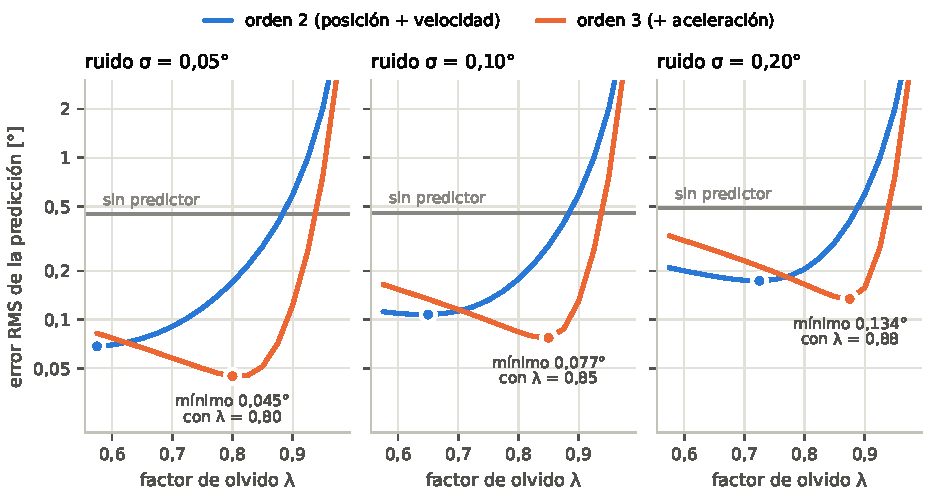
\includegraphics[width=\linewidth]{pred_error_lambda.pdf}
\caption{Error RMS de la predicción a 20~ms según $\lam$, para un objetivo senoidal de $20\gr$ de amplitud y
0,25~Hz (velocidad máxima $31\gr$/s, aceleración máxima $49\gr$/s$^2$). La línea gris es no predecir: usar la
última medición. Eje vertical logarítmico. Como referencia, $0{,}115\gr$ equivalen a 1~px.}
\label{fig:error}
\end{figure}

\begin{table}[H]
\centering\small
\caption{Mejor $\lam$ según el ruido de la medición, para el objetivo de la figura~\ref{fig:error}.}
\label{tab:mejor}
\setlength{\tabcolsep}{4pt}
\begin{tabular}{@{}cccccc@{}}
\toprule
Ruido $\sigma$ & Equivale a & Sin predictor & Mejor orden 2 & \textbf{Mejor orden 3} & Orden 3 con $\lam = 0{,}80$ \\
\midrule
$0{,}05\gr$ & 0,4 px & $0{,}45\gr$ & $0{,}07\gr$ ($\lam \le 0{,}60$) & $\mathbf{0{,}045\gr}$ ($\lam = 0{,}80$) & $0{,}045\gr$ \\
$0{,}10\gr$ & 0,9 px & $0{,}46\gr$ & $0{,}11\gr$ ($\lam = 0{,}65$) & $\mathbf{0{,}077\gr}$ ($\lam = 0{,}85$) & $0{,}084\gr$ \\
$0{,}20\gr$ & 1,7 px & $0{,}49\gr$ & $0{,}17\gr$ ($\lam = 0{,}72$) & $\mathbf{0{,}134\gr}$ ($\lam = 0{,}88$) & $0{,}165\gr$ \\
\bottomrule
\end{tabular}
\end{table}

Tres conclusiones:
\begin{itemize}
  \item El orden 3 con $\lam$ entre 0,80 y 0,88 es la mejor combinación en los tres niveles de ruido. La
        decisión del informe del 25~\% (orden 3, $\lam = 0{,}80$) sigue siendo correcta.
  \item El mínimo es ancho hacia la izquierda y abrupto hacia la derecha. Equivocarse hacia $\lam$ bajo cuesta
        poco; pasarse de 0,90 cuesta mucho, y con 0,95 el predictor es \emph{peor} que no predecir.
  \item Con orden 3 no conviene bajar de 0,60: la predicción amplifica el ruido (ganancia 1,54) y la traza de
        $\mathbf P$ se acerca al tope de $10^6$ de \cod{\_sanear()}, que empieza a actuar cerca de $\lam = 0{,}5$.
        El tablero limita $\lam$ al rango de 0,60 a 0,99.
\end{itemize}

% ------------------------------------------------------------------------------------------
\section{Hallazgos de la revisión del código}
\label{sec:hallazgos}

\subsection{El predictor de posición, solo, mueve poco la aguja}

Se corrió el lazo cerrado simulado (\cod{main.py --enlace simulado}, 10~s a 80~cuadros/s, objetivo de hasta
$24{,}7\gr$/s con dos oclusiones) barriendo $\lam$ y el orden, con y sin feedforward.

\begin{figure}[H]
\centering
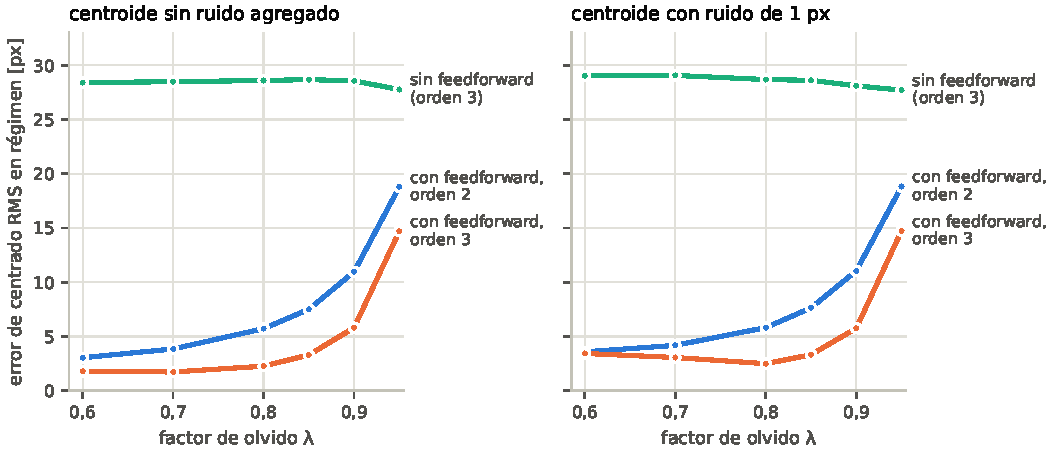
\includegraphics[width=\linewidth]{pred_lazo_cerrado.pdf}
\caption{Error de centrado RMS en los tramos de seguimiento sin oclusión (1 a 2,9~s y 7 a 10~s), en lazo cerrado
simulado. Sin feedforward, el orden 2 da la misma curva plana que el orden 3 (no se dibuja).}
\label{fig:lc}
\end{figure}

\begin{table}[H]
\centering\small
\caption{Lazo cerrado simulado, orden 3, sin ruido agregado al centroide. Error de centrado RMS en píxeles.}
\label{tab:lc}
\begin{tabular}{@{}lcccccc@{}}
\toprule
 & \multicolumn{6}{c}{$\lam$} \\
\cmidrule(l){2-7}
Configuración & 0,60 & 0,70 & 0,80 & 0,85 & 0,90 & 0,95 \\
\midrule
Sin feedforward, en régimen     & 28,4 & 28,5 & 28,6 & 28,7 & 28,6 & 27,8 \\
Con feedforward, en régimen     & 1,8  & 1,7  & \textbf{2,3} & 3,3 & 5,8 & 14,7 \\
Sin feedforward, toda la corrida & 31,9 & 31,7 & 31,6 & 31,6 & 31,5 & 32,4 \\
Con feedforward, toda la corrida & 12,2 & 11,4 & \textbf{11,2} & 11,6 & 12,1 & 17,7 \\
\bottomrule
\end{tabular}
\end{table}

\begin{itemize}
  \item \textbf{Sin feedforward, cambiar $\lam$ no cambia nada.} El error en régimen es de 28 a 29~px (unos
        $3{,}3\gr$) para cualquier valor. Sin predictor ni feedforward, usando la última medición, la corrida
        completa da 35,3~px: el predictor de posición sólo aporta un 10~\%.
  \item \textbf{La causa.} Adelantar la referencia 20~ms corrige $0{,}5\gr$ a $25\gr$/s. El atraso del lazo de
        posición es mucho mayor: con la ganancia de arranque de pan ($K_p = 3$~s$^{-1}$), seguir un objetivo a
        $20\gr$/s sólo con la acción proporcional exige un error de $20/3 \approx 6{,}7\gr$. El integrador lo
        reduce, pero lento, y sólo integra con $|e| < 5\gr$.
  \item \textbf{Con feedforward el error en régimen baja 12 veces}, de 28,6 a 2,3~px. Ahí $\lam$ sí importa,
        y el óptimo queda entre 0,70 y 0,80, igual que en la figura~\ref{fig:error}.
  \item Con 1~px de ruido agregado al centroide el resultado es el mismo: 28,7~px sin feedforward y 2,5~px con
        feedforward, orden 3 y $\lam = 0{,}80$.
\end{itemize}

El feedforward está apagado por defecto (\cod{usar\_feedforward = False}; se activa con \cod{--feedforward}).
Si la prueba de lazo cerrado se hizo sin esa opción, lo observado calza con esta simulación: el predictor
funciona, pero su efecto queda tapado por el atraso del lazo interno.

\subsection{Un reinicio del estimador pasa por PÉRDIDA}

Cuando el gating rechaza tres mediciones seguidas, \cod{EstimadorEje} se reinicia (\cod{prediccion.py}, líneas
48 a 56). El estimador nuevo no está \cod{listo()} hasta juntar 3 muestras, y mientras tanto
\cod{Estimador2D} entrega confianza 0 (líneas 126 y 127). El supervisor lee esa confianza y pasa de
SEGUIMIENTO a PÉRDIDA. Al simular un salto de $3\gr$ en la medición, la secuencia fue:

\begin{itemize}
  \item 3 cuadros (37~ms) con la medición rechazada: la referencia sigue la trayectoria vieja;
  \item 1 cuadro en PÉRDIDA: la consigna se retiene y \cod{main.py} reinicia la ventana del detector, que
        vuelve a buscar en el cuadro completo;
  \item vuelta a SEGUIMIENTO en el cuadro siguiente, todavía con el estimador a medio llenar.
\end{itemize}

No es grave, pero es un tirón visible, y al volver al cuadro completo el detector puede engancharse en otra
mancha. Ocurre cada vez que la detección salta más de $0{,}6\gr$ (5~px), algo esperable con el avión, cuya
mancha cambia de forma al girar.

\subsection{Otros puntos}

\begin{itemize}
  \item \textbf{El gating es independiente por eje.} Un mismo cuadro puede ser aceptado en pan y rechazado en
        tilt. Una detección falsa suele estar mal en los dos ejes, así que conviene decidir en conjunto.
  \item \textbf{La confianza sólo mira el eje pan.} \cod{Estimador2D} usa \cod{self.eu} para \cod{listo()} y para
        el tiempo sin medición (líneas 124 a 126). Si tilt está rechazando mediciones, la confianza no lo refleja.
  \item \textbf{En oclusión se extrapola con aceleración.} Con orden 3, el error de extrapolar crece con el
        cuadrado del tiempo. Con $\sigma = 0{,}10\gr$ y $\lam = 0{,}80$, a 300~ms la dispersión simulada es de
        $0{,}64\gr$ con orden 3 y de $0{,}16\gr$ con orden 2. La plataforma sigue esa extrapolación hasta
        300~ms (\cod{t\_perdida\_s}).
  \item \textbf{La medición depende de la sincronía.} La dirección en el mundo usa $\theta_{\mathrm{med}}$ en el
        instante de la foto. El tiempo de lectura del sensor (\cod{t\_lectura\_ms} $= 12$) es una estimación sin
        medir. Con la plataforma a $30\gr$/s, cada milisegundo de error son $0{,}03\gr$ de movimiento propio que
        el predictor toma por movimiento del objetivo.
  \item \textbf{Comentario desactualizado.} El encabezado de \cod{rls\_predictor.py} dice que $s$ es del orden de
        16,7~ms (60~cuadros/s). Hoy son 12,5~ms.
\end{itemize}

% ------------------------------------------------------------------------------------------
\newpage
\section{Ajustes sugeridos}
\label{sec:ajustes}

Ordenados por efecto esperado. Los tres primeros no tocan código: se hacen desde el tablero.

\begin{table}[H]
\small
\renewcommand{\arraystretch}{1.25}
\begin{tabularx}{\linewidth}{@{}c>{\raggedright\arraybackslash}p{3.5cm}>{\raggedright\arraybackslash}X>{\raggedright\arraybackslash}p{3.6cm}@{}}
\toprule
\# & Ajuste & Por qué & Cómo \\
\midrule
1 & Activar el feedforward de velocidad & En simulación baja el error en régimen de 28,6 a 2,3~px. Es el mayor efecto disponible. & Tablero: casilla ``Feedforward'', o \cod{--feedforward} \\
2 & Medir el ruido real $\sigma$ de la medición & $\lam$ se elige según $\sigma$ (tabla~\ref{tab:mejor}), y hoy $\sigma$ sólo se conoce en simulación. & Procedimiento de abajo \\
3 & Partir con $\lam = 0{,}80$ y probar hasta 0,88 & Rango óptimo del orden 3. Subir si los motores suenan ásperos con feedforward; no pasar de 0,90. & Tablero: deslizador de $\lam$ \\
4 & Reinicio sin pasar por PÉRDIDA & Evita el tirón y la pérdida de la ventana del detector en cada salto de la detección. & Código, \cod{prediccion.py} \\
5 & Gating conjunto y confianza con ambos ejes & Una detección falsa se rechaza completa; la confianza refleja a tilt. & Código, \cod{prediccion.py} \\
6 & En oclusión, extrapolar sin aceleración & Dispersión cuatro veces menor a 300~ms. & Código, \cod{prediccion.py} \\
7 & Prueba de sincronía & Detecta errores de tiempo entre cámara y AS5600, que con feedforward pueden hacer oscilar el lazo. & Procedimiento de abajo \\
8 & Piso del gating por objetivo & $0{,}1\gr$ sirve para el láser; el avión probablemente necesita más. & Tablero: ``Piso del gating''; se guarda en el perfil \\
\bottomrule
\end{tabularx}
\end{table}

\textbf{Sobre el ajuste 1.} El feedforward usa la velocidad estimada, que es más ruidosa que la posición. Con
orden 3 y $\lam = 0{,}80$ el ruido de $\omega_{\mathrm{ff}}$ es $12 \times \sigma$: unos $0{,}6\gr$/s si
$\sigma = 0{,}05\gr$. Si resulta mucho, $\lam = 0{,}85$ lo baja a $7{,}3 \times \sigma$. Conviene activarlo
primero con un objetivo lento y alguien a cargo del corte.

\textbf{Procedimiento para medir $\sigma$ (ajuste 2).} Objetivo fijo, plataforma habilitada y quieta, 10~s de
registro. $\sigma$ es la desviación estándar de las columnas \cod{pan\_obj} y \cod{tilt\_obj} del CSV. Repetir
con cada objetivo (láser, luz, avión): el del avión debería ser el mayor.

\textbf{Procedimiento de sincronía (ajuste 7).} Objetivo fijo (láser en la pared) y la plataforma moviéndose,
por ejemplo con escalones de referencia desde la consola del ESP32. La columna \cod{pan\_obj} debería quedar
constante. Si oscila al ritmo del movimiento, hay un error de tiempo: su valor es la variación de
\cod{pan\_obj} dividida por la velocidad \cod{esp32\_w\_pan}. Se corrige con \cod{t\_lectura\_ms}.

\textbf{Qué mirar en el registro para diagnosticar.}
\begin{itemize}
  \item \cod{est\_u} y \cod{est\_w}: fracción de \cod{rechazada} durante SEGUIMIENTO. Sobre 1 o 2~\%, el gating
        está apretado o la detección salta.
  \item Bitácora del supervisor: transiciones a PÉRDIDA con causa \cod{confianza 0.00} son reinicios del estimador.
  \item \cod{h\_ms}: horizonte real de cada cuadro (mediana y percentil 95).
  \item \cod{lam} y \cod{detector}: valores vigentes en cada fila, ahora que se pueden cambiar en vivo.
\end{itemize}

% ------------------------------------------------------------------------------------------
\newpage
\section{Resumen en palabras sencillas, para presentar}

\begin{lamina}{1. El problema}
La cámara siempre muestra el pasado. Desde que saca la foto hasta que el motor recibe la orden pasan unos
20 milisegundos. Si el objetivo se mueve, cuando la plataforma llega a donde lo vio, ya no está ahí.
\end{lamina}

\begin{lamina}{2. La idea}
Es lo que hace alguien que atrapa una pelota: no estira la mano hacia donde la ve, sino hacia donde va a
estar. El predictor mira las últimas posiciones del objetivo, calcula su velocidad y su aceleración, y con eso
estima dónde estará 20 milisegundos después. Esa posición futura es la que se le manda al motor.
\end{lamina}

\begin{lamina}{3. Cómo lo hace}
Ajusta una curva suave a las últimas posiciones medidas y la prolonga un poco hacia adelante. Las mediciones
recientes pesan más que las antiguas. En cada foto nueva corrige la curva en vez de calcularla de nuevo, por
eso es rápido: se llama mínimos cuadrados recursivos (RLS).
\end{lamina}

\begin{lamina}{4. La perilla: el factor de olvido $\lam$}
$\lam$ decide cuánta memoria tiene el predictor.
\begin{itemize}
  \item \textbf{Memoria larga} ($\lam$ alto): promedia muchas fotos. Es estable frente al ruido, pero tarda en
        darse cuenta de que el objetivo cambió de rumbo.
  \item \textbf{Memoria corta} ($\lam$ bajo): reacciona al instante, pero se cree cada temblor de la medición.
\end{itemize}
Usamos $\lam = 0{,}80$: recuerda unas 5 fotos, es decir 60 milisegundos.
\end{lamina}

\begin{lamina}{5. Las protecciones}
\begin{itemize}
  \item Si una medición sale absurda (un reflejo, otra luz), se descarta.
  \item Si el objetivo se tapa, el predictor sigue estimando por dónde va, y su confianza baja con el tiempo.
        Pasados 0,3 segundos el sistema declara el objetivo perdido y la plataforma se queda quieta.
\end{itemize}
\end{lamina}

\begin{lamina}{6. Qué tan bien funciona y qué falta}
En simulación, predecir reduce el error de apuntar unas diez veces frente a usar la última foto. En las
pruebas de lazo cerrado esa mejora todavía se nota poco. La simulación indica por qué: el lazo de los
motores responde más lento que el predictor. El paso siguiente es mandarle al motor también la \emph{velocidad} que estima el predictor: en simulación eso
baja el error de centrado de 28 a 2 píxeles.
\end{lamina}

\textbf{Si preguntan por qué RLS y no un filtro de Kalman.} El RLS con olvido no necesita un modelo del ruido
del objetivo ni de la medición: tiene una sola perilla, $\lam$. En régimen equivale a un filtro $\alpha$-$\beta$-$\gamma$, que es un
filtro de Kalman de ganancia fija, y cuesta unos 0,05~ms por cuadro en un PC.

\textbf{Si preguntan por qué orden 3.} Con velocidad constante (orden 2) el predictor se atrasa cada vez que el
objetivo acelera o cambia de sentido. Agregar la aceleración elimina ese atraso; a cambio deja pasar algo más
de ruido, que se compensa con un $\lam$ un poco mayor.

\end{document}
